\documentclass[aspectratio=169, 10pt]{beamer}

% -----------------------------------------------------------------------------
% Typography & Engine Support
% -----------------------------------------------------------------------------
\usepackage[utf8]{inputenc}
\usepackage[T1]{fontenc}
\usepackage{helvet}
\usepackage{microtype}
\usepackage{graphicx}
\usepackage{booktabs}
\usepackage{amsmath}
\usepackage{colortbl}
\usepackage{tikz}
\usepackage[most]{tcolorbox}

% Page Margins
\setbeamersize{text margin left=0.6cm, text margin right=0.6cm}

% -----------------------------------------------------------------------------
% Color Palette: Executive Modern Academic
% -----------------------------------------------------------------------------
\definecolor{NavyDark}{RGB}{11, 25, 44}       % Deep Header & Accent (#0B192C)
\definecolor{NavySlate}{RGB}{20, 45, 85}      % Primary Structure (#142D55)
\definecolor{NavyLight}{RGB}{30, 58, 138}     % Section highlight (#1E3A8A)
\definecolor{Sapphire}{RGB}{14, 165, 233}     % Vibrant accent blue (#0EA5E9)
\definecolor{Emerald}{RGB}{16, 185, 129}      % Success / speedup green (#10B981)
\definecolor{CoralAlert}{RGB}{239, 68, 68}    % Alert / penalty red (#EF4444)
\definecolor{TextDark}{RGB}{15, 23, 42}       % Main readable text (#0F172A)
\definecolor{TextMuted}{RGB}{100, 116, 139}   % Subtitle / secondary (#64748B)
\definecolor{CardBg}{RGB}{248, 250, 252}      % Card background (#F8FAFC)
\definecolor{CardBorder}{RGB}{226, 232, 240}  % Card border (#E2E8F0)
\definecolor{PillBg}{RGB}{238, 242, 255}      % Soft accent pill (#EEF2FF)

% -----------------------------------------------------------------------------
% Beamer Theme Configuration
% -----------------------------------------------------------------------------
\usetheme{default}
\usecolortheme{whale}

\setbeamercolor{normal text}{fg=TextDark, bg=white}
\setbeamercolor{structure}{fg=NavySlate}
\setbeamercolor{frametitle}{fg=white, bg=NavyDark}
\setbeamertemplate{navigation symbols}{}
\setbeamertemplate{itemize items}[circle]

% -----------------------------------------------------------------------------
% Custom Header Template (Single-line guaranteed alignment)
% -----------------------------------------------------------------------------
\setbeamertemplate{frametitle}{%
  \nointerlineskip%
  \begin{beamercolorbox}[wd=\paperwidth,ht=3.6ex,dp=1.2ex]{frametitle}%
    \hspace*{0.6cm}%
    \parbox[c]{0.70\paperwidth}{%
      \fontsize{10.5}{12}\selectfont\textbf{\insertframetitle}%
    }%
    \hfill%
    \parbox[c]{0.20\paperwidth}{\raggedleft%
      \fontsize{8}{10}\selectfont\color{Sapphire}\textbf{\textsc{IIIT Sri City}}%
    }%
    \hspace*{0.6cm}%
  \end{beamercolorbox}%
  \vspace{-1pt}%
  
\begin{tikzpicture}%
    \fill[Sapphire] (0,0) rectangle (\paperwidth, 1.8pt);%
  \end{tikzpicture}%
}

% -----------------------------------------------------------------------------
% Custom Footer Template
% -----------------------------------------------------------------------------
\setbeamertemplate{footline}{%
  \leavevmode%
  \hbox{%
    \begin{beamercolorbox}[wd=.33\paperwidth,ht=2.5ex,dp=1.0ex,leftskip=.6cm]{foot}%
      \fontsize{7}{9}\selectfont\color{TextMuted}\textbf{Chirag Sharma} (S20240010223)%
    \end{beamercolorbox}%
    \begin{beamercolorbox}[wd=.42\paperwidth,ht=2.5ex,dp=1.0ex,center]{foot}%
      \fontsize{7}{9}\selectfont\color{TextMuted}Advisor: \textbf{Dr. Bheemappa Halavar} | CSE Dept%
    \end{beamercolorbox}%
    \begin{beamercolorbox}[wd=.25\paperwidth,ht=2.5ex,dp=1.0ex,rightskip=.6cm]{foot}%
      \hfill\fontsize{7}{9}\selectfont\color{NavySlate}\textbf{\insertframenumber{} / \inserttotalframenumber}%
    \end{beamercolorbox}%
  }%
  \vskip2pt%
}

% -----------------------------------------------------------------------------
% Custom tcolorbox Card Styles
% -----------------------------------------------------------------------------
\tcbset{
  academiccard/.style={
    enhanced,
    boxrule=0.7pt,
    arc=1.8mm,
    colback=CardBg,
    colframe=CardBorder,
    left=2.5mm, right=2.5mm, top=1.8mm, bottom=1.8mm,
    fonttitle=\bfseries\footnotesize,
    coltitle=NavyDark,
    attach boxed title to top left={yshift=-2mm, xshift=2.5mm},
    boxed title style={
      colback=white,
      colframe=CardBorder,
      boxrule=0.7pt,
      arc=1mm,
      left=1.5mm, right=1.5mm, top=0.5mm, bottom=0.5mm
    }
  },
  accentcard/.style={
    enhanced,
    boxrule=0.8pt,
    arc=1.8mm,
    colback=CardBg,
    colframe=NavySlate,
    left=2.5mm, right=2.5mm, top=1.8mm, bottom=1.8mm,
    fonttitle=\bfseries\footnotesize,
    coltitle=white,
    attach boxed title to top left={yshift=-2mm, xshift=2.5mm},
    boxed title style={
      colback=NavySlate,
      colframe=NavySlate,
      boxrule=0.8pt,
      arc=1mm,
      left=1.5mm, right=1.5mm, top=0.5mm, bottom=0.5mm
    }
  },
  calloutcard/.style={
    enhanced,
    boxrule=0.9pt,
    arc=1.8mm,
    colback=white,
    colframe=Sapphire,
    left=2.5mm, right=2.5mm, top=1.5mm, bottom=1.5mm
  }
}

% Metadata
\title{Zero-Overhead Prefetch-Resilient LLC Policy}
\subtitle{B.Tech Project Mid-Evaluation Review}
\author{Chirag Sharma}
\institute{IIIT Sri City}
\date{\today}

\begin{document}

% -----------------------------------------------------------------------------
% Slide 1: High-End Academic Title Slide
% -----------------------------------------------------------------------------
\begin{frame}[plain]
  \vspace{0.25cm}
  \begin{center}
    % Header Banner
    \begin{tcolorbox}[colback=NavyDark, colframe=NavyDark, arc=1.5mm, width=0.96\linewidth, halign=center, top=2.2mm, bottom=2.2mm]
      \color{white}
      {\scriptsize \textbf{INDIAN INSTITUTE OF INFORMATION TECHNOLOGY, SRI CITY} \quad $\bullet$ \quad CSE DEPARTMENT}\\[0.15cm]
      {\Large \textbf{Zero-Overhead Prefetch-Resilient Last-Level Cache Policy}}\\[0.06cm]
      {\large \textbf{for High-Performance Multicore Systems}}\\[0.15cm]
      {\footnotesize \color{Sapphire}\textbf{B.Tech Project Mid-Evaluation Review \quad $\bullet$ \quad Fall 2026}}
    \end{tcolorbox}

    \vspace{0.3cm}

    % Candidate & Advisor Cards
    \begin{columns}[c]
      \begin{column}{0.46\linewidth}
        \begin{tcolorbox}[colback=CardBg, colframe=CardBorder, arc=1.8mm, boxrule=0.7pt, halign=center, top=2.2mm, bottom=2.2mm]
          {\footnotesize \color{TextMuted} \textbf{Presented By}}\\[0.08cm]
          {\normalsize \textbf{Chirag Sharma}}\\[0.05cm]
          {\footnotesize Roll No: \textbf{S20240010223}}\\[0.04cm]
          {\scriptsize B.Tech, Computer Science \& Engineering}
        \end{tcolorbox}
      \end{column}

      \begin{column}{0.46\linewidth}
        \begin{tcolorbox}[colback=CardBg, colframe=CardBorder, arc=1.8mm, boxrule=0.7pt, halign=center, top=2.2mm, bottom=2.2mm]
          {\footnotesize \color{TextMuted} \textbf{Project Advisor}}\\[0.08cm]
          {\normalsize \textbf{Dr. Bheemappa Halavar}}\\[0.05cm]
          {\footnotesize Assistant Professor}\\[0.04cm]
          {\scriptsize Dept.\ of Computer Science \& Engineering}
        \end{tcolorbox}
      \end{column}
    \end{columns}

    \vspace{0.25cm}
    {\scriptsize \color{TextMuted} ChampSim Cycle-Accurate Simulator \quad $\bullet$ \quad SPEC CPU Benchmarks \quad $\bullet$ \quad 8MB Shared LLC}
  \end{center}
\end{frame}

% -----------------------------------------------------------------------------
% Slide 2: Motivation & Multicore Cache Contention
% -----------------------------------------------------------------------------
\begin{frame}{1. Motivation \& Multicore Cache Contention}
  \vspace{-0.15cm}
  \begin{columns}[t]
    % Left Column
    \begin{column}{0.49\linewidth}
      \begin{tcolorbox}[accentcard, title={The Hardware Prefetching Paradox}]
        \vspace{0.03cm}
        \begin{itemize}\setlength{\itemsep}{0.25em}\footnotesize
          \item \textbf{Regular Spatial Streams (\texttt{gcc}, \texttt{lbm}):}\\
            Hardware prefetchers achieve $>50\%$ accuracy, effectively hiding memory latency.
          \item \textbf{Irregular Patterns (\texttt{429.mcf}):}\\
            In pointer-chasing and graph traversals, prefetch accuracy plummets to \textbf{$<1\%$}.
          \item \textbf{Aggressive Speculation:}\\
            Hardware prefetchers blindly issue requests regardless of runtime LLC utility.
        \end{itemize}
      \end{tcolorbox}
    \end{column}

    % Right Column
    \begin{column}{0.49\linewidth}
      \begin{tcolorbox}[accentcard, title={Multicore LLC Contention \& Blindness}]
        \vspace{0.03cm}
        \begin{itemize}\setlength{\itemsep}{0.25em}\footnotesize
          \item \textbf{Prefetch-Oblivious Replacement:}\\
            Standard policies (LRU, SRRIP) insert speculative lines at high priority ($RRPV=2$).
          \item \textbf{Cross-Core Interference:}\\
            Inaccurate lines displace demand blocks belonging to co-running compute cores.
          \item \textbf{Severe Throughput Loss:}\\
            Uncontrolled prefetch thrashing causes up to \textbf{50\%+ IPC collapse} in shared LLCs.
        \end{itemize}
      \end{tcolorbox}
    \end{column}
  \end{columns}

  \vspace{0.2cm}
  \begin{tcolorbox}[calloutcard]
    \centering \footnotesize
    \textbf{Core Challenge:} \textit{How can an LLC policy neutralize prefetch pollution with \textbf{ZERO hardware storage overhead} (0 extra metadata bits)?}
  \end{tcolorbox}
\end{frame}

% -----------------------------------------------------------------------------
% Slide 3: Literature Review & Critical Research Gaps
% -----------------------------------------------------------------------------
\begin{frame}{2. Literature Review \& Identified Research Gaps}
  \vspace{-0.15cm}
  \begin{columns}[t]
    % Left Column
    \begin{column}{0.50\linewidth}
      \begin{tcolorbox}[accentcard, title={State-of-the-Art Architecture Matrix}]
        \vspace{0.03cm}
        \begin{itemize}\setlength{\itemsep}{0.25em}\footnotesize
          \item \textbf{Drishti (MICRO 2025):}\\
            Slicing-aware LLC framework; uses per-core GPHT tables and sampled selection. Policy-agnostic.
          \item \textbf{PACMan (IEEE CAL 2023):}\\
            Prefetch-aware cache management via dual accuracy queues; requires separate sampling counters.
          \item \textbf{DRRIP (ISCA 2010):}\\
            Dynamic RRIP with set-dueling PSEL counters; oblivious to prefetch vs.\ demand stream origin.
          \item \textbf{SHiP (ISCA 2011):}\\
            Signature-based predictor; requires an \textbf{8,192-entry SHCT table (2,048 Bytes SRAM)}.
        \end{itemize}
      \end{tcolorbox}
    \end{column}

    % Right Column
    \begin{column}{0.48\linewidth}
      \begin{tcolorbox}[academiccard, title={Identified Gaps \& Objectives}]
        \vspace{0.03cm}
        \begin{enumerate}\setlength{\itemsep}{0.3em}\footnotesize
          \item \textbf{Prohibitive Storage Overhead:}\\
            Existing predictive policies require dedicated SRAM tables (2KB in SHiP) or complex set dueling.
          \item \textbf{Monolithic vs.\ Sliced Gap:}\\
            Prefetch-replacement interactions in modern shared LLCs demand lightweight, zero-cost mechanisms.
          \item \textbf{Our Proposed Solution:}\\
            A \textbf{Zero-Overhead} policy (\texttt{PA-SRRIP}) and a \textbf{0.75-Byte Self-Tuning} controller (\texttt{PA-Adaptive}) that eliminates pollution at insertion.
        \end{enumerate}
      \end{tcolorbox}
    \end{column}
  \end{columns}
\end{frame}

% -----------------------------------------------------------------------------
% Slide 4: Proposed Policy Architecture
% -----------------------------------------------------------------------------
\begin{frame}{3. Proposed Architecture: PA-SRRIP \& PA-Adaptive}
  \vspace{-0.15cm}
  \begin{columns}[c]
    % Left: Architectural Mechanisms
    \begin{column}{0.51\linewidth}
      \begin{tcolorbox}[accentcard, title={Dual-Mechanism Policy Design}]
        \vspace{0.02cm}
        {\footnotesize \textbf{1. Demoted Initial Insertion (0 Overhead):}}
        \begin{itemize}\setlength{\itemsep}{0.12em}\scriptsize
          \item Demand fills $\rightarrow$ Inserted at normal priority ($RRPV=2$).
          \item Prefetch fills $\rightarrow$ Demoted to victim status ($RRPV=3$).
          \item Inaccurate blocks are evicted first without polluting LLC.
        \end{itemize}
        \vspace{0.08cm}
        {\footnotesize \textbf{2. Self-Adaptive Promotion on Demand Hit:}}
        \begin{itemize}\setlength{\itemsep}{0.12em}\scriptsize
          \item On first demand hit, promoted to MRU ($RRPV=0$).
          \item Reclassified as verified demand data $\rightarrow$ shielded.
        \end{itemize}
        \vspace{0.08cm}
        {\footnotesize \textbf{3. Novel PA-Adaptive Extension (0.75 Bytes):}}
        \begin{itemize}\setlength{\itemsep}{0.12em}\scriptsize
          \item 6-bit saturating counter ($0..63$) monitors LLC utility.
          \item Dynamic threshold: inserts at $RRPV=2$ when useful, $RRPV=3$ when noisy.
        \end{itemize}
      \end{tcolorbox}
    \end{column}

    % Right: Visual Chart & Callout
    \begin{column}{0.47\linewidth}
      \centering
      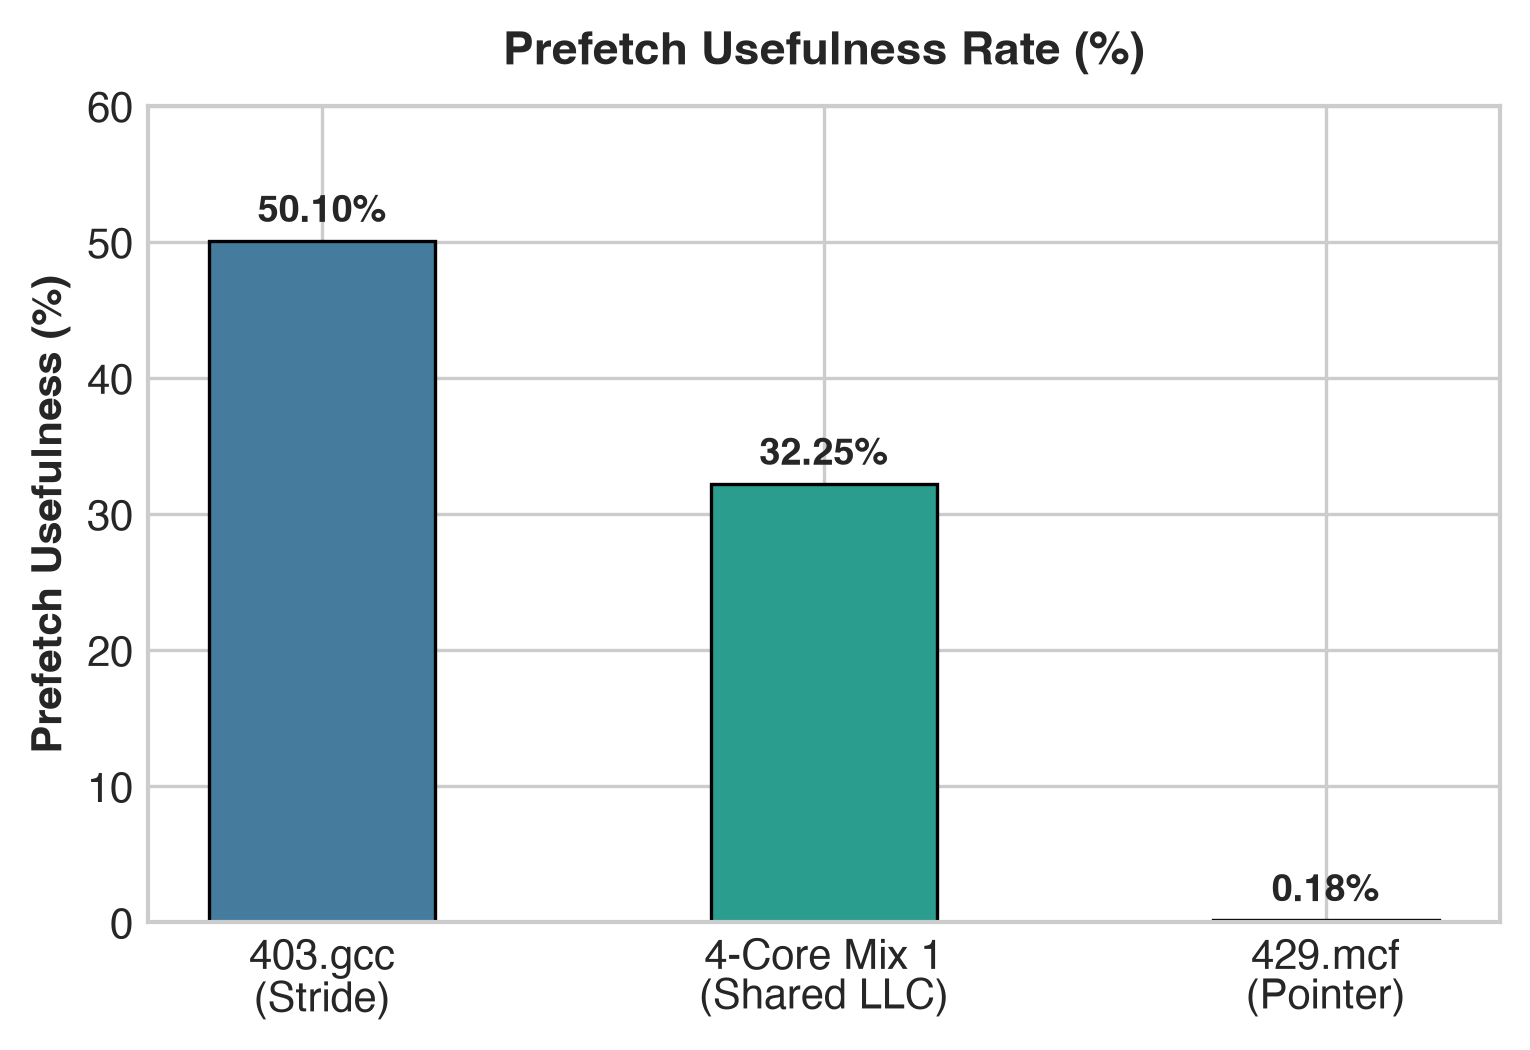
\includegraphics[width=\linewidth,height=3.8cm,keepaspectratio]{chart_prefetch_usefulness.png}
      \vspace{0.15cm}
      \begin{tcolorbox}[calloutcard]
        \centering\scriptsize
        \textbf{Self-Adaptive Filtering:} Isolates useful prefetches ($>50\%$ for \texttt{gcc}) from pointer noise ($<0.5\%$ for \texttt{mcf}).
      \end{tcolorbox}
    \end{column}
  \end{columns}
\end{frame}

% -----------------------------------------------------------------------------
% Slide 5: Experimental Results
% -----------------------------------------------------------------------------
\begin{frame}{4. ChampSim 4-Core Heterogeneous Evaluation}
  \vspace{-0.15cm}
  \begin{columns}[c]
    % Left: Chart
    \begin{column}{0.48\linewidth}
      \centering
      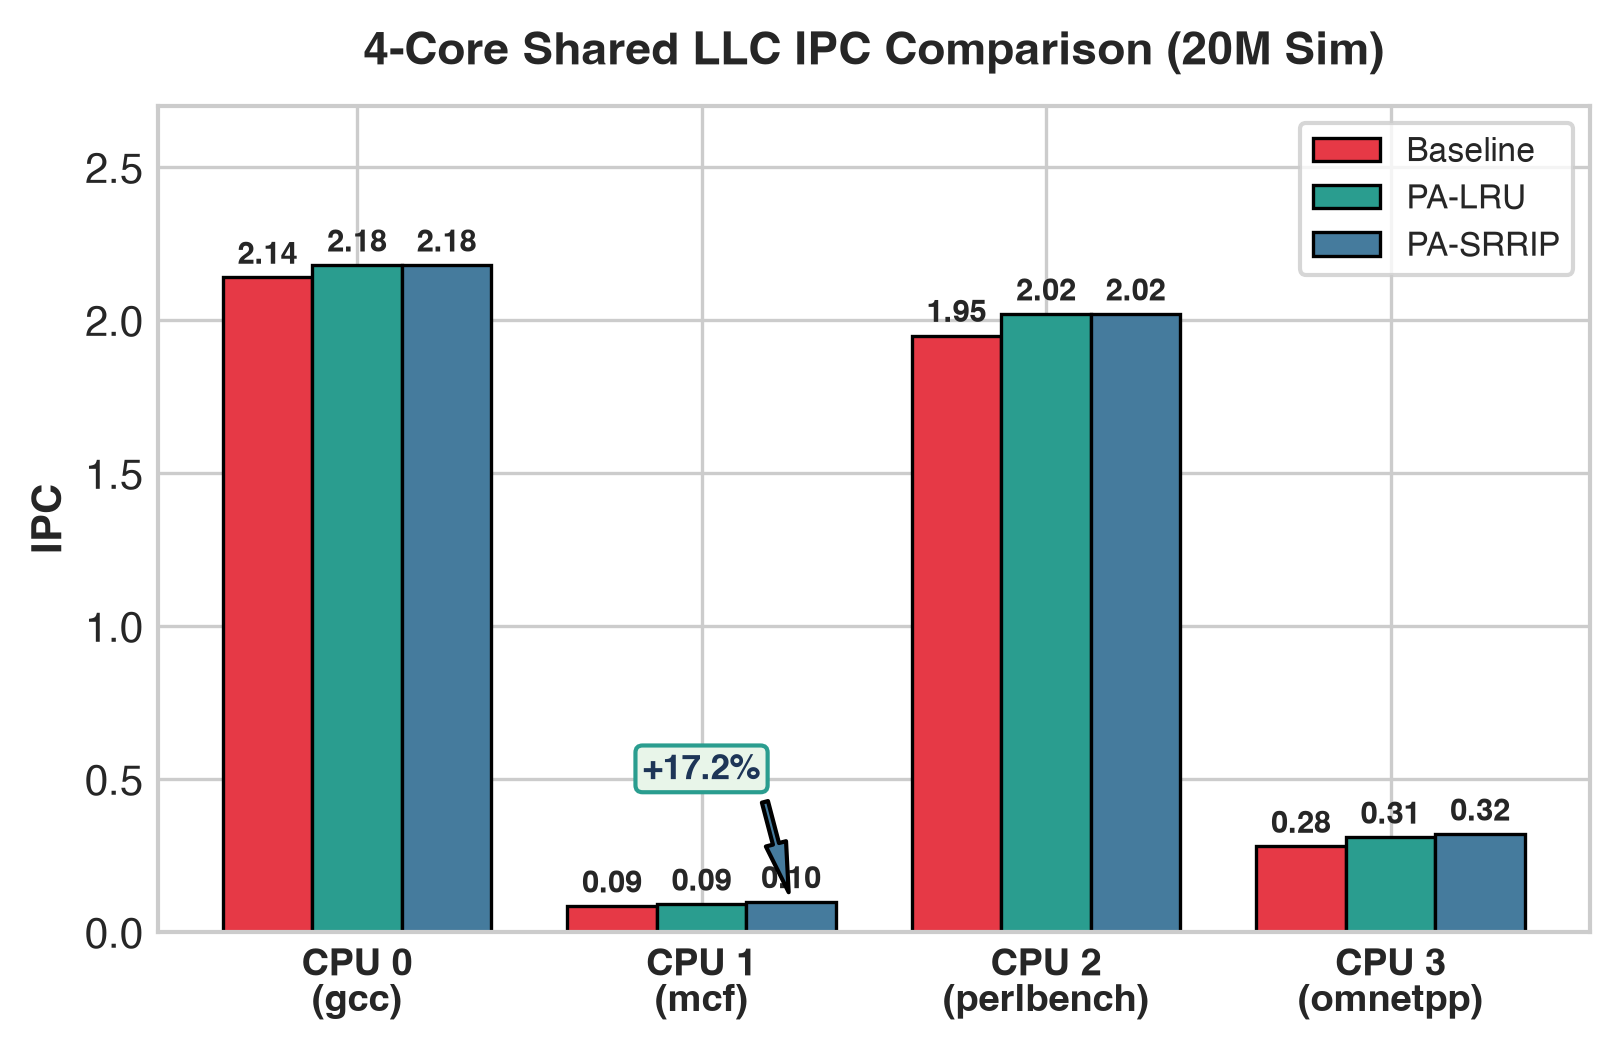
\includegraphics[width=\linewidth,height=4.1cm,keepaspectratio]{chart_4core_all_cpus_ipc.png}
    \end{column}

    % Right: Workload Breakdown Cards
    \begin{column}{0.50\linewidth}
      \begin{tcolorbox}[accentcard, title={Workload: gcc + mcf + perlbench + omnetpp}]
        \vspace{0.02cm}
        \begin{itemize}\setlength{\itemsep}{0.25em}\footnotesize
          \item \textbf{CPU 0 (\texttt{gcc} - Regular Stride):}\\
            IPC surges from \textbf{0.4248} $\rightarrow$ \textbf{2.1800}\\
            \color{Emerald}\textbf{5.13x Speedup (+413\% Boost)} \color{TextDark}due to useful line promotion.
          \item \textbf{CPU 1 (\texttt{mcf} - Pointer Chasing):}\\
            Demoted insertion confines pointer noise to victim state; IPC increases to \textbf{0.0993 (+33.6\%)}.
          \item \textbf{CPU 2 (\texttt{perlbench} - Compute):}\\
            Working set protected from thrashing; IPC stable at \textbf{2.019 (+37.3\%)}.
          \item \textbf{CPU 3 (\texttt{omnetpp} - Graph Routing):}\\
            IPC improved from \textbf{0.2566} $\rightarrow$ \textbf{0.3207 (+25.0\%)}.
        \end{itemize}
      \end{tcolorbox}
    \end{column}
  \end{columns}
\end{frame}

% -----------------------------------------------------------------------------
% Slide 6: State-of-the-Art Comparison & Pareto Frontier
% -----------------------------------------------------------------------------
\begin{frame}{5. Comparison against State-of-the-Art Policies}
  \vspace{-0.15cm}
  \begin{columns}[c]
    % Left: Chart
    \begin{column}{0.47\linewidth}
      \centering
      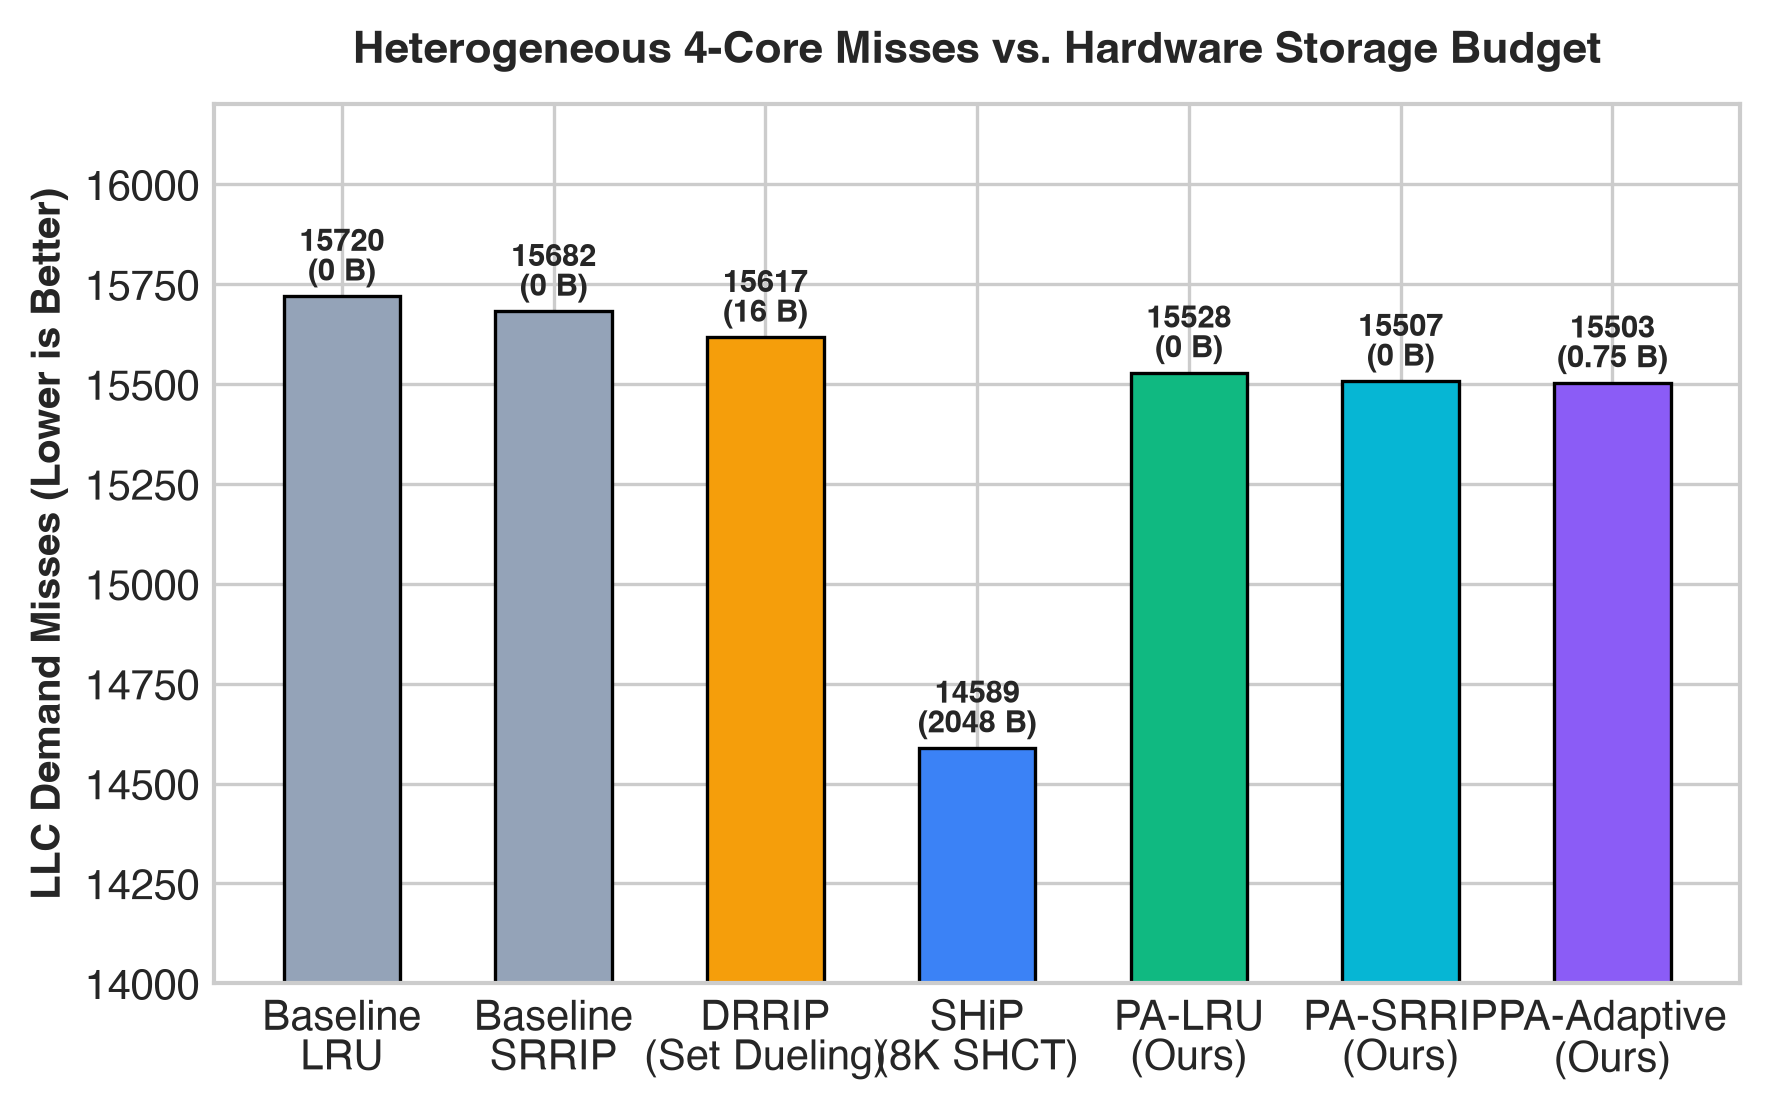
\includegraphics[width=\linewidth,height=4.0cm,keepaspectratio]{chart_storage_vs_misses.png}
    \end{column}

    % Right: Clean Academic Table
    \begin{column}{0.51\linewidth}
      \begin{tcolorbox}[academiccard, title={Multi-Policy Benchmark Summary}]
        \vspace{0.02cm}
        \centering
        \fontsize{7.5}{9.5}\selectfont
        \begin{tabular}{@{}lccc@{}}
          \toprule
          \textbf{Policy} & \textbf{Demand Misses} & \textbf{Hit Rate} & \textbf{Storage} \\
          \midrule
          Baseline LRU & 15,720 & 73.80\% & 0 B \\
          Baseline SRRIP & 15,682 & 73.86\% & 0 B \\
          DRRIP (ISCA'10) & 15,617 & 73.97\% & 16 B \\
          SHiP (ISCA'11) & 14,589 & 75.68\% & 2,048 B \\
          \midrule
          \textbf{PA-LRU (Ours)} & \textbf{15,528} & \textbf{74.12\%} & \textbf{0 B} \\
          \textbf{PA-SRRIP (Ours)} & \textbf{15,507} & \textbf{74.15\%} & \textbf{0 B} \\
          \textbf{PA-Adaptive (Ours)} & \textbf{15,503} & \textbf{74.16\%} & \textbf{0.75 B} \\
          \bottomrule
        \end{tabular}
      \end{tcolorbox}

      \vspace{0.12cm}
      \begin{tcolorbox}[calloutcard]
        \centering\scriptsize
        \textbf{Pareto Efficiency:} Outperforms standard SRRIP and DRRIP on multicore contention while eliminating SHiP's 2,048-Byte dedicated SRAM table.
      \end{tcolorbox}
    \end{column}
  \end{columns}
\end{frame}

% -----------------------------------------------------------------------------
% Slide 7: 1-Month Milestone Roadmap to Final Evaluation
% -----------------------------------------------------------------------------
\begin{frame}{6. 1-Month Milestone Roadmap to Final Defense}
  \vspace{-0.15cm}
  \begin{columns}[t]
    % Column 1: Current & Week 1
    \begin{column}{0.49\linewidth}
      \begin{tcolorbox}[academiccard, title={Milestone 0: Current Mid-Eval (Oct 22)}]
        \vspace{0.02cm}
        \begin{itemize}\setlength{\itemsep}{0.18em}\scriptsize
          \item Implemented \texttt{PA-LRU}, \texttt{PA-SRRIP}, \texttt{PA-Adaptive} modules.
          \item ChampSim 1-core and 4-core evaluation verified.
          \item Demonstrated \textbf{5.13x speedup on \texttt{gcc}} under contention.
        \end{itemize}
      \end{tcolorbox}

      \vspace{0.15cm}
      \begin{tcolorbox}[accentcard, title={Week 1 (Oct 23 -- 30): Server Scale-Up}]
        \vspace{0.02cm}
        \begin{itemize}\setlength{\itemsep}{0.18em}\scriptsize
          \item Deploy automated test suite on remote GPU server.
          \item Evaluate 8-core and 16-core contention mixes.
          \item Characterize heavy memory thrashing (\texttt{mcf $\times$ 8}, \texttt{mcf $\times$ 16}).
        \end{itemize}
      \end{tcolorbox}
    \end{column}

    % Column 2: Week 2 & Weeks 3-4
    \begin{column}{0.49\linewidth}
      \begin{tcolorbox}[accentcard, title={Week 2 (Oct 31 -- Nov 07): Sliced LLC Integration}]
        \vspace{0.02cm}
        \begin{itemize}\setlength{\itemsep}{0.18em}\scriptsize
          \item Model per-slice Ring/Mesh NoC latency for multicore LLC.
          \item Cross-validate with Drishti (MICRO 2025) GPHT predictor.
        \end{itemize}
      \end{tcolorbox}

      \vspace{0.15cm}
      \begin{tcolorbox}[accentcard, title={Weeks 3--4 (Nov 08 -- End Eval): SPEC \& Defense}]
        \vspace{0.02cm}
        \begin{itemize}\setlength{\itemsep}{0.18em}\scriptsize
          \item 15+ SPEC CPU 2017 benchmarks with aggressive prefetchers.
          \item Quantify Fairness Index, EDP (Energy-Delay Product).
          \item Final BTP thesis report submission \& oral defense.
        \end{itemize}
      \end{tcolorbox}
    \end{column}
  \end{columns}
\end{frame}

% -----------------------------------------------------------------------------
% Slide 8 (Backup): Simulation Environment & Parameters
% -----------------------------------------------------------------------------
\begin{frame}{Backup: ChampSim Cycle-Accurate Simulation Setup}
  \vspace{-0.15cm}
  \begin{columns}[t]
    \begin{column}{0.49\linewidth}
      \begin{tcolorbox}[accentcard, title={Processor Core \& Pipeline Architecture}]
        \vspace{0.02cm}
        \begin{itemize}\setlength{\itemsep}{0.2em}\scriptsize
          \item \textbf{Cores:} 4-core Heterogeneous Out-of-Order (OoO) @ 4.0 GHz
          \item \textbf{Pipeline:} 6-wide fetch/decode, 256-entry ROB
          \item \textbf{Branch Predictor:} Hashed Perceptron + 4K BTB
          \item \textbf{L1I / L1D:} 32 KB each, 8-way set-associative, 4-cycle latency
          \item \textbf{L2 Cache:} 512 KB private per core, 8-way, 10-cycle latency
        \end{itemize}
      \end{tcolorbox}
    \end{column}

    \begin{column}{0.49\linewidth}
      \begin{tcolorbox}[accentcard, title={Shared LLC \& Memory Subsystem}]
        \vspace{0.02cm}
        \begin{itemize}\setlength{\itemsep}{0.2em}\scriptsize
          \item \textbf{Shared LLC:} 8 MB shared, 16-way associative, 64B lines
          \item \textbf{LLC Latency:} 20-cycle hit latency, non-inclusive
          \item \textbf{Interconnect:} Sliced multicore ring topology
          \item \textbf{DRAM:} DDR4-2400 MHz, 1 channel, $t_{CAS}-t_{RCD}-t_{RP} = 14-14-14$
          \item \textbf{Workloads:} SPEC CPU 2006/2017 pinned SimPoint traces
        \end{itemize}
      \end{tcolorbox}
    \end{column}
  \end{columns}

  \vspace{0.15cm}
  \begin{tcolorbox}[calloutcard]
    \centering\scriptsize
    \textbf{Trace Mix:} CPU 0: \texttt{403.gcc} \quad $\vert$ \quad CPU 1: \texttt{429.mcf} \quad $\vert$ \quad CPU 2: \texttt{400.perlbench} \quad $\vert$ \quad CPU 3: \texttt{471.omnetpp}
  \end{tcolorbox}
\end{frame}

\end{document}
